%%%%%%%%%%%%%%%%%%%%%%%%%%%
% Inflated Expectations
% Cassandra Grafström and Christopher Gandrud
% 9 May 2014
%%%%%%%%%%%%%%%%%%%%%%%%%%%%

% !Rnw weave = knitr

\documentclass[a4paper]{article}\usepackage[]{graphicx}\usepackage[]{color}
%% maxwidth is the original width if it is less than linewidth
%% otherwise use linewidth (to make sure the graphics do not exceed the margin)
\makeatletter
\def\maxwidth{ %
  \ifdim\Gin@nat@width>\linewidth
    \linewidth
  \else
    \Gin@nat@width
  \fi
}
\makeatother

\definecolor{fgcolor}{rgb}{0.345, 0.345, 0.345}
\newcommand{\hlnum}[1]{\textcolor[rgb]{0.686,0.059,0.569}{#1}}%
\newcommand{\hlstr}[1]{\textcolor[rgb]{0.192,0.494,0.8}{#1}}%
\newcommand{\hlcom}[1]{\textcolor[rgb]{0.678,0.584,0.686}{\textit{#1}}}%
\newcommand{\hlopt}[1]{\textcolor[rgb]{0,0,0}{#1}}%
\newcommand{\hlstd}[1]{\textcolor[rgb]{0.345,0.345,0.345}{#1}}%
\newcommand{\hlkwa}[1]{\textcolor[rgb]{0.161,0.373,0.58}{\textbf{#1}}}%
\newcommand{\hlkwb}[1]{\textcolor[rgb]{0.69,0.353,0.396}{#1}}%
\newcommand{\hlkwc}[1]{\textcolor[rgb]{0.333,0.667,0.333}{#1}}%
\newcommand{\hlkwd}[1]{\textcolor[rgb]{0.737,0.353,0.396}{\textbf{#1}}}%

\usepackage{framed}
\makeatletter
\newenvironment{kframe}{%
 \def\at@end@of@kframe{}%
 \ifinner\ifhmode%
  \def\at@end@of@kframe{\end{minipage}}%
  \begin{minipage}{\columnwidth}%
 \fi\fi%
 \def\FrameCommand##1{\hskip\@totalleftmargin \hskip-\fboxsep
 \colorbox{shadecolor}{##1}\hskip-\fboxsep
     % There is no \\@totalrightmargin, so:
     \hskip-\linewidth \hskip-\@totalleftmargin \hskip\columnwidth}%
 \MakeFramed {\advance\hsize-\width
   \@totalleftmargin\z@ \linewidth\hsize
   \@setminipage}}%
 {\par\unskip\endMakeFramed%
 \at@end@of@kframe}
\makeatother

\definecolor{shadecolor}{rgb}{.97, .97, .97}
\definecolor{messagecolor}{rgb}{0, 0, 0}
\definecolor{warningcolor}{rgb}{1, 0, 1}
\definecolor{errorcolor}{rgb}{1, 0, 0}
\newenvironment{knitrout}{}{} % an empty environment to be redefined in TeX

\usepackage{alltt}
\usepackage{fullpage}
\usepackage[authoryear]{natbib}
\usepackage{setspace}
    \doublespacing
\usepackage{hyperref}
\hypersetup{
    colorlinks,
    citecolor=black,
    filecolor=black,
    linkcolor=cyan,
    urlcolor=cyan
}
\usepackage{dcolumn}
\usepackage{booktabs}
\usepackage{url}
\usepackage{tikz}
\usepackage{todonotes}
\usepackage[utf8]{inputenc}
\usepackage{graphicx}

% Set knitr global options






%%%%%%% Title Page %%%%%%%%%%%%%%%%%%%%%%%%%%%%%%%%%%%%%%%%%%%%
\title{Supplemental Materials for: Inflated Expectations: How government partisanship shapes monetary policy bureaucrats' inflation forecasts}

\author{Christopher Gandrud \\
                {\emph{Hertie School of Governance}}\footnote{Post-doctoral Fellow. Friedrichstra{\ss}e 180. 10117 Berlin, Germany. Email: \href{mailto:gandrud@hertie-school.org}{gandrud@hertie-school.org}.} \\
                and \\
            Cassandra Grafstr\"{o}m \\
                {\emph{University of Michigan}}\footnote{Ph.D Candidate. 5700 Haven Hall, 505 S. State Street
                Ann Arbor, MI 48109-1045. USA. Email: \href{mailto:cgrafstr@umich.edu}{cgrafstr@umich.edu}.} \footnote{Thank you to the Mark Hallerberg and the Fiscal Governance Centre at the Hertie School of Governance for comments and support. Thank you also to Leonardo Baccini, Vincent Arel-Bundock, Mark Kayser, Cheryl Schonhardt-Bailey, Tom Stark, and seminar participants at the Hertie School of Governance, London School of Economics, and Yonsei University as well as two anonymous reviewers.}}
\IfFileExists{upquote.sty}{\usepackage{upquote}}{}

\begin{document}

\maketitle


In the Supplementary Materials we present additional robustness checks to further test the strength of our main empirical findings.

\subsection*{Mid-term election timing}

To further check the robustness of the possible effect of elections on errors we examined models with election variables that included mid-term elections--non-presidential elections when the House of Representatives and a portion of the Senate is elected--in addition to presidential elections. As before, we subsetted the data to exclude quarters when the forecasters would not have known who the winners of the elections would be. This variable was, like the equivalent variable that only included presidential election timing, statistically insignificant. Its interaction with presidential party ID was also insignificant. Table \ref{MidTerm} shows results from two of these models.

\begin{table}[ht]
    \caption{Normal Linear Regression Estimation with Standardized 2 Qrt. Inflation Forecasting Error as the Dependent Variable and a Quarter to Election Variables that Included Midterms (non-matched data set)}
    \label{MidTerm}
    \vspace{0.25cm}
    \begin{center}
    {\small{
 
\begin{tabular}{ l D{.}{.}{1}D{.}{.}{1} } 
\hline 
  & \multicolumn{ 1 }{ c }{ SM1 } & \multicolumn{ 1 }{ c }{ SM2 } \\ \hline
 %                                & SM1             & SM2            \\ 
Intercept                        & -0.2            & -0.2           \\ 
                                 & (2.2)           & (2.2)          \\ 
Recession                        & 0.0             & 0.0            \\ 
                                 & (0.1)           & (0.1)          \\ 
Expenditure/GDP                  & 0.1 ^{***}      & 0.1 ^{***}     \\ 
                                 & (0.0)           & (0.0)          \\ 
Output Gap                       & -0.0            & -0.0           \\ 
                                 & (0.0)           & (0.0)          \\ 
Discount Rate Change             & -0.3 ^{**}      & -0.3 ^{**}     \\ 
                                 & (0.1)           & (0.1)          \\ 
Unemployment Rate                & -0.1 ^\dagger  & -0.1 ^\dagger \\ 
                                 & (0.0)           & (0.0)          \\ 
Pres. Party ID                   & 0.3 ^{***}      & 0.3 ^{***}     \\ 
                                 & (0.0)           & (0.1)          \\ 
Qrt. Midterm/Pres. Election      & 0.0             & 0.0            \\ 
                                 & (0.0)           & (0.0)          \\ 
FRB/GlobalModel                  & 0.1             & 0.1            \\ 
                                 & (0.1)           & (0.1)          \\ 
Senate Dem/Rep                   & -0.4 ^*         & -0.4 ^*        \\ 
                                 & (0.2)           & (0.2)          \\ 
House Dem/Rep                    & 0.4 ^*          & 0.4 ^*         \\ 
                                 & (0.2)           & (0.2)          \\ 
Pres*Qrt. Midterm/Pres. Election &                 & 0.0            \\ 
                                 &                 & (0.0)           \\
 $N$                              & 115             & 115            \\ 
AIC                              & -39.0           & -37.0          \\ 
BIC                              & 81.8            & 94.8           \\ 
$\log L$                        & 63.5            & 66.5            \\ \hline
 \multicolumn{3}{l}{\footnotesize{Standard errors in parentheses}}\\
\multicolumn{3}{l}{\footnotesize{$^\dagger$ significant at $p<.10$; $^* p<.05$; $^{**} p<.01$; $^{***} p<.001$}} 
\end{tabular} 


    }}
    \end{center}
\end{table}

\subsection*{President party ID and election timing linear interaction}

In the body of the paper we presented results from models with president party ID and the square of quarters to the election. The first model in Table \ref{SupTable1} shows results with an interaction between president party ID and the non-squared linear version of election timing. The results are substantively equivalent to those with the squared version. In both cases the interaction is not statistically significant.

\subsection*{Economic and violent conflict shocks}

We examined if economic and/or violent conflict shocks may affect inflation forecast errors. First we examined if the underlying level of inflation could impact the standardized forecast errors. Perhaps if price changes are very volatile, e.g. inflation is very high, then there may be larger errors. We examined this possibility by including two absolute inflation variables in the models: (a) the \textbf{absolute inflation level in the quarter being forecasted} for and (b) \textbf{absolute inflation in the quarter prior} to when the forecast was made.\footnote{In Table \ref{SupTable1} this is referred to as `Lag 3 Abs. Inflation'.} The second and third models in Table \ref{SupTable1} show that including these variables did not substantively change the presidential partisan ID results. Absolute inflation in the quarter being forecasted for has a statistically significant negative relationship with forecast errors. Referring back to figures 2 and 3 in the main paper, this makes empirical sense as periods of high inflation in the 1970s were actually times when the standardized forecast error was relatively small. This finding persists even if we use absolute inflation forecast errors (i.e. $F_{q} - I_{q}$) as the dependent variable. This can be seen in Model S14 in Table \ref{SupTable2}.

We also interacted the absolute inflation variables with presidential party ID. In both cases we estimated that there are small though statistically significant interaction terms. The interaction terms and absolute inflation coefficient estimates are negative, while presidential partisan ID remains positive. Again returning to figures \ref{absolute} and \ref{errors_over_time}, this finding makes sense as the period of high absolute inflation with a Democratic president (Carter) was a time of low standardized forecast errors.

We consider other economic and political shocks. Perhaps oil price shocks, for example in the late 1970s, increased inflation forecast errors. To examine this possibility we gathered data from the FRED database on the \textbf{change in the West Texas Crude price}\footnote{The series ID is OILPRICE. Accessed October 2013.} from the quarter in the previous year to the quarter the inflation forecast was made for. Similarly, maybe labor productivity increases, especially in the 1990s, created unexpected economic conditions that dampened inflation, changing inflation forecasting errors. To examine this possibility we gathered data from the United States Bureau of Labor Statistics on non-farm business \textbf{labor productivity}.\footnote{The series ID was PR85006092. Accessed October 2013.} The variable is in terms of the percent change from the previous quarter at the annual rate. Finally, perhaps violent conflict also created unexpected economic conditions. To examine this we created an indicator of the \textbf{total number of armed conflicts per year that the United States participated in} using data from the Uppsala Conflict Data Program/Peace Research Institute Oslo \citep{Harbom2008,Themner2013}.

We can see in tables \ref{SupTable1} and \ref{SupTable2} that productivity changes were not robustly associated with inflation forecasting errors. Oil price changes were found to be statistically significantly associated with errors. This association was negative so that high price increases are related to lower errors. This mirrors our finding for the absolute inflation level. High absolute inflation and high oil price increases are associated in time during our observation period. They were both particularly high during the mid to late 1970s. This was simultaneously a period of relatively small to negative inflation forecast errors. The number of armed conflicts that the US participated in was found to be significantly negatively associated with inflation forecast errors. This result is being driven by the fact that a long period of inflation under estimates--primarily during George W. Bush's presidency--also was the period where the United States engaged in the most armed conflicts as part of the so-called `War on Terror'. This evidence suggests that Fed staff do not overestimate the effect that price, oil, and armed conflict shocks have on inflation, though they may underestimate their effects.

In Table~\ref{SupTable1} we also included interactions between presidential party ID and the oil price, productivity, and armed conflict shock variables. None of these interactions were estimated to be statistically significant.

Overall, it is important to note that the presidential partisan ID variable's estimated effect largely does not change in magnitude, direction, or statistical significance when the shock variables are included. It also doesn't change when we use our standardized measure or inflation forecasting errors or absolute errors (results shown in Table~\ref{SupTable2}).

\begin{table}[ht]
    \caption{Normal Linear Regression Estimation with Standardized 2 Qtr. Inflation Forecasting Error as the Dependent Variable and Additional Independent Variables (non-matched data set)}
    \label{SupTable1}
    \vspace{0.25cm}
    \begin{center}
    {\tiny{
 
\begin{tabular}{ l D{.}{.}{1}D{.}{.}{1}D{.}{.}{1}D{.}{.}{1}D{.}{.}{1}D{.}{.}{1}D{.}{.}{1}D{.}{.}{1}D{.}{.}{1}D{.}{.}{1}D{.}{.}{1} } 
\hline 
  & \multicolumn{ 1 }{ c }{ S1 } & \multicolumn{ 1 }{ c }{ S2 } & \multicolumn{ 1 }{ c }{ S3 } & \multicolumn{ 1 }{ c }{ S4 } & \multicolumn{ 1 }{ c }{ S5 } & \multicolumn{ 1 }{ c }{ S6 } & \multicolumn{ 1 }{ c }{ S7 } & \multicolumn{ 1 }{ c }{ S8 } & \multicolumn{ 1 }{ c }{ S9 } & \multicolumn{ 1 }{ c }{ S10 } & \multicolumn{ 1 }{ c }{ S11 } \\ \hline
 %                     & S1              & S2              & S3              & S4              & S5              & S6              & S7              & S8              & S9              & S10             & S11            \\ 
Intercept             & 2.0             & 2.3             & 3.0             & 1.4             & 2.4             & 2.2             & 2.1             & 2.3             & 2.2             & -0.4            & -0.5           \\ 
                      & (2.0)           & (1.9)           & (1.9)           & (2.1)           & (2.1)           & (1.9)           & (1.9)           & (2.0)           & (1.9)           & (1.8)           & (1.8)          \\ 
Recession             & 0.0             & 0.1 ^*          & 0.1 ^*          & 0.1             & 0.1             & 0.1             & 0.1             & 0.0             & 0.0             & -0.0            & -0.0           \\ 
                      & (0.1)           & (0.1)           & (0.1)           & (0.1)           & (0.1)           & (0.1)           & (0.1)           & (0.1)           & (0.1)           & (0.1)           & (0.1)          \\ 
Expenditure/GDP       & 0.1 ^{***}      & 0.1 ^{***}      & 0.1 ^{***}      & 0.1 ^{***}      & 0.1 ^{***}      & 0.1 ^{***}      & 0.1 ^{***}      & 0.1 ^{***}      & 0.1 ^{***}      & 0.1 ^{***}      & 0.1 ^{***}     \\ 
                      & (0.0)           & (0.0)           & (0.0)           & (0.0)           & (0.0)           & (0.0)           & (0.0)           & (0.0)           & (0.0)           & (0.0)           & (0.0)          \\ 
Output Gap            & -0.0 ^*         & -0.0 ^*         & -0.1 ^*         & -0.0            & -0.0 ^*         & -0.0 ^*         & -0.0 ^*         & -0.0 ^*         & -0.0 ^*         & -0.0            & -0.0           \\ 
                      & (0.0)           & (0.0)           & (0.0)           & (0.0)           & (0.0)           & (0.0)           & (0.0)           & (0.0)           & (0.0)           & (0.0)           & (0.0)          \\ 
Discount Rate Change  & -0.3 ^{**}      & -0.2 ^\dagger  & -0.2 ^*         & -0.3 ^{**}      & -0.3 ^{**}      & -0.2 ^*         & -0.2 ^\dagger  & -0.3 ^{**}      & -0.3 ^{**}      & -0.1            & -0.1           \\ 
                      & (0.1)           & (0.1)           & (0.1)           & (0.1)           & (0.1)           & (0.1)           & (0.1)           & (0.1)           & (0.1)           & (0.1)           & (0.1)          \\ 
Unemployment Rate     & -0.1            & -0.0            & -0.0            & -0.1            & -0.0            & -0.1            & -0.1            & -0.1            & -0.1            & -0.1 ^{**}      & -0.1 ^{**}     \\ 
                      & (0.0)           & (0.0)           & (0.0)           & (0.0)           & (0.0)           & (0.0)           & (0.0)           & (0.0)           & (0.0)           & (0.0)           & (0.0)          \\ 
FRB/GlobalModel       & 0.1             & 0.1 ^*          & 0.1 ^\dagger   & 0.1 ^\dagger   & 0.1 ^\dagger   & 0.1             & 0.1             & 0.1 ^\dagger   & 0.1 ^\dagger   & 0.0             & 0.0            \\ 
                      & (0.1)           & (0.1)           & (0.1)           & (0.1)           & (0.1)           & (0.1)           & (0.1)           & (0.1)           & (0.1)           & (0.1)           & (0.1)          \\ 
Senate Dem/Rep        & -0.3 ^*         & -0.3 ^*         & -0.3 ^*         & -0.4 ^*         & -0.3 ^*         & -0.3 ^*         & -0.3 ^\dagger  & -0.4 ^*         & -0.3 ^*         & -0.5 ^{***}     & -0.5 ^{***}    \\ 
                      & (0.2)           & (0.1)           & (0.1)           & (0.2)           & (0.1)           & (0.1)           & (0.2)           & (0.1)           & (0.1)           & (0.1)           & (0.1)          \\ 
House Dem/Rep         & 0.3 ^*          & 0.4 ^{**}       & 0.4 ^{**}       & 0.3 ^*          & 0.4 ^*          & 0.3 ^*          & 0.3 ^*          & 0.3 ^*          & 0.3 ^*          & 0.4 ^{***}      & 0.4 ^{**}      \\ 
                      & (0.1)           & (0.1)           & (0.1)           & (0.1)           & (0.1)           & (0.1)           & (0.1)           & (0.1)           & (0.1)           & (0.1)           & (0.1)          \\ 
Pres. Party ID        & 0.3 ^{***}      & 0.3 ^{***}      & 0.4 ^{***}      & 0.3 ^{***}      & 0.4 ^{***}      & 0.3 ^{***}      & 0.3 ^{***}      & 0.3 ^{***}      & 0.3 ^{***}      & 0.1 ^*          & 0.1 ^*         \\ 
                      & (0.1)           & (0.0)           & (0.1)           & (0.0)           & (0.1)           & (0.0)           & (0.0)           & (0.0)           & (0.0)           & (0.0)           & (0.0)          \\ 
Qtr. to Election      & 0.0             & 0.0             &                 &                 &                 &                 &                 &                 &                 &                 &                \\ 
                      & (0.0)           & (0.0)           &                 &                 &                 &                 &                 &                 &                 &                 &                \\ 
Pres*Qrt. Election    & -0.0            &                 &                 &                 &                 &                 &                 &                 &                 &                 &                \\ 
                      & (0.0)           &                 &                 &                 &                 &                 &                 &                 &                 &                 &                \\ 
Abs. Inflation        &                 & -0.0 ^{**}      & -0.0            &                 &                 &                 &                 &                 &                 &                 &                \\ 
                      &                 & (0.0)           & (0.0)           &                 &                 &                 &                 &                 &                 &                 &                \\ 
Pres*Abs. Infl.       &                 &                 & -0.0 ^*         &                 &                 &                 &                 &                 &                 &                 &                \\ 
                      &                 &                 & (0.0)           &                 &                 &                 &                 &                 &                 &                 &                \\ 
Lag 3 Abs. Inflation  &                 &                 &                 & -0.0            & -0.0            &                 &                 &                 &                 &                 &                \\ 
                      &                 &                 &                 & (0.0)           & (0.0)           &                 &                 &                 &                 &                 &                \\ 
Pres*Lag 3 Abs. Infl. &                 &                 &                 &                 & -0.0 ^*         &                 &                 &                 &                 &                 &                \\ 
                      &                 &                 &                 &                 & (0.0)           &                 &                 &                 &                 &                 &                \\ 
Oil Price Change      &                 &                 &                 &                 &                 & -0.0 ^\dagger  & -0.0 ^\dagger  &                 &                 &                 &                \\ 
                      &                 &                 &                 &                 &                 & (0.0)           & (0.0)           &                 &                 &                 &                \\ 
Pres*Oil Price Change &                 &                 &                 &                 &                 &                 & 0.0             &                 &                 &                 &                \\ 
                      &                 &                 &                 &                 &                 &                 & (0.0)           &                 &                 &                 &                \\ 
Productivity Change   &                 &                 &                 &                 &                 &                 &                 & -0.0            & -0.0            &                 &                \\ 
                      &                 &                 &                 &                 &                 &                 &                 & (0.0)           & (0.0)           &                 &                \\ 
Pres*Prod. Change     &                 &                 &                 &                 &                 &                 &                 &                 & 0.0             &                 &                \\ 
                      &                 &                 &                 &                 &                 &                 &                 &                 & (0.0)           &                 &                \\ 
No. Armed Conflicts   &                 &                 &                 &                 &                 &                 &                 &                 &                 & -0.1 ^{***}     & -0.1 ^{***}    \\ 
                      &                 &                 &                 &                 &                 &                 &                 &                 &                 & (0.0)           & (0.0)          \\ 
Pres*No. Armed Confl. &                 &                 &                 &                 &                 &                 &                 &                 &                 &                 & 0.1            \\ 
                      &                 &                 &                 &                 &                 &                 &                 &                 &                 &                 & (0.1)           \\
 $N$                   & 135             & 135             & 135             & 132             & 132             & 135             & 135             & 135             & 135             & 135             & 135            \\ 
AIC                   & -55.3           & -64.8           & -69.4           & -53.9           & -58.5           & -60.9           & -59.0           & -57.4           & -58.0           & -83.4           & -81.9          \\ 
BIC                   & 84.2            & 74.7            & 70.1            & 72.9            & 79.8            & 66.9            & 80.4            & 70.4            & 81.4            & 44.5            & 57.5           \\ 
$\log L$             & 75.6            & 80.4            & 82.7            & 71.0            & 77.3            & 74.4            & 77.5            & 72.7            & 77.0            & 85.7            & 89.0            \\ \hline
 \multicolumn{12}{l}{\footnotesize{Standard errors in parentheses}}\\
\multicolumn{12}{l}{\footnotesize{$^\dagger$ significant at $p<.10$; $^* p<.05$; $^{**} p<.01$; $^{***} p<.001$}} 
\end{tabular} 


    }}
    \end{center}
\end{table}


\begin{table}[ht]
    \caption{Normal Linear Regression Estimation with Absolute 2 Qtr. Inflation Forecasting Error as the Dependent Variable and Additional Independent Variables (non-matched data set)}
    \label{SupTable2}
    \vspace{0.25cm}
    \begin{center}
    {\tiny{
 
\begin{tabular}{ l D{.}{.}{1}D{.}{.}{1}D{.}{.}{1}D{.}{.}{1}D{.}{.}{1}D{.}{.}{1}D{.}{.}{1}D{.}{.}{1} } 
\hline 
  & \multicolumn{ 1 }{ c }{ S12 } & \multicolumn{ 1 }{ c }{ S13 } & \multicolumn{ 1 }{ c }{ S14 } & \multicolumn{ 1 }{ c }{ S15 } & \multicolumn{ 1 }{ c }{ S16 } & \multicolumn{ 1 }{ c }{ S17 } & \multicolumn{ 1 }{ c }{ S18 } & \multicolumn{ 1 }{ c }{ S19 } \\ \hline
 %                    & S12             & S13             & S14             & S15             & S16             & S17             & S18             & S19            \\ 
Intercept            & 3.1             & 3.0             & 3.3 ^\dagger   & 2.3             & 3.3 ^\dagger   & 3.3             & 0.5             & 0.8            \\ 
                     & (2.0)           & (2.0)           & (1.9)           & (2.1)           & (1.9)           & (2.0)           & (1.8)           & (1.9)          \\ 
Recession            & 0.1             & 0.0             & 0.1 ^*          & 0.1             & 0.1             & 0.0             & -0.0            & 0.0            \\ 
                     & (0.1)           & (0.1)           & (0.1)           & (0.1)           & (0.1)           & (0.1)           & (0.1)           & (0.1)          \\ 
Expenditure/GDP      & 0.1 ^{***}      & 0.1 ^{***}      & 0.1 ^{***}      & 0.1 ^{***}      & 0.1 ^{***}      & 0.1 ^{***}      & 0.1 ^{***}      & 0.1 ^{***}     \\ 
                     & (0.0)           & (0.0)           & (0.0)           & (0.0)           & (0.0)           & (0.0)           & (0.0)           & (0.0)          \\ 
Output Gap           & -0.0 ^*         & -0.0 ^*         & -0.0 ^*         & -0.0            & -0.0 ^*         & -0.0 ^*         & -0.0            & -0.0           \\ 
                     & (0.0)           & (0.0)           & (0.0)           & (0.0)           & (0.0)           & (0.0)           & (0.0)           & (0.0)          \\ 
Discount Rate Change & -0.3 ^{**}      & -0.3 ^{**}      & -0.2 ^\dagger  & -0.3 ^{**}      & -0.2 ^*         & -0.3 ^{**}      & -0.1            & -0.1           \\ 
                     & (0.1)           & (0.1)           & (0.1)           & (0.1)           & (0.1)           & (0.1)           & (0.1)           & (0.1)          \\ 
Unemployment Rate    & -0.1            & -0.1            & -0.0            & -0.1            & -0.1            & -0.1            & -0.1 ^{**}      & -0.1 ^{**}     \\ 
                     & (0.0)           & (0.0)           & (0.0)           & (0.0)           & (0.0)           & (0.0)           & (0.0)           & (0.0)          \\ 
Pres. Party ID       & 0.3 ^{***}      & 0.3 ^{***}      & 0.3 ^{***}      & 0.3 ^{***}      & 0.3 ^{***}      & 0.3 ^{***}      & 0.1 ^*          & 0.1 ^*         \\ 
                     & (0.0)           & (0.1)           & (0.0)           & (0.0)           & (0.0)           & (0.0)           & (0.0)           & (0.0)          \\ 
Qtr. to Election     & 0.0             & 0.0             & 0.0             & 0.0             & -0.0            & 0.0             & 0.0             & -0.0           \\ 
                     & (0.0)           & (0.0)           & (0.0)           & (0.0)           & (0.0)           & (0.0)           & (0.0)           & (0.0)          \\ 
FRB/GlobalModel      & 0.1 ^\dagger   & 0.1             & 0.1 ^*          & 0.1 ^\dagger   & 0.1             & 0.1             & 0.0             & 0.0            \\ 
                     & (0.1)           & (0.1)           & (0.1)           & (0.1)           & (0.1)           & (0.1)           & (0.1)           & (0.1)          \\ 
Senate Dem/Rep       & -0.4 ^*         & -0.3 ^*         & -0.3 ^*         & -0.4 ^*         & -0.3 ^*         & -0.4 ^*         & -0.5 ^{***}     & -0.5 ^{***}    \\ 
                     & (0.1)           & (0.2)           & (0.1)           & (0.2)           & (0.1)           & (0.2)           & (0.1)           & (0.1)          \\ 
House Dem/Rep        & 0.3 ^*          & 0.3 ^*          & 0.4 ^{**}       & 0.3 ^*          & 0.3 ^*          & 0.3 ^*          & 0.4 ^{***}      & 0.4 ^{**}      \\ 
                     & (0.1)           & (0.1)           & (0.1)           & (0.1)           & (0.1)           & (0.1)           & (0.1)           & (0.1)          \\ 
Pres*Qrt. Election   &                 & -0.0            &                 &                 &                 &                 &                 &                \\ 
                     &                 & (0.0)           &                 &                 &                 &                 &                 &                \\ 
Abs Inflation        &                 &                 & -0.0 ^{**}      &                 &                 &                 &                 &                \\ 
                     &                 &                 & (0.0)           &                 &                 &                 &                 &                \\ 
Lag 3 Abs. Inflation &                 &                 &                 & -0.0            &                 &                 &                 &                \\ 
                     &                 &                 &                 & (0.0)           &                 &                 &                 &                \\ 
Oil Price Change     &                 &                 &                 &                 & -0.0 ^\dagger  &                 &                 & -0.0           \\ 
                     &                 &                 &                 &                 & (0.0)           &                 &                 & (0.0)          \\ 
Productivity Change  &                 &                 &                 &                 &                 & -0.0            &                 & -0.0           \\ 
                     &                 &                 &                 &                 &                 & (0.0)           &                 & (0.0)          \\ 
No. Armed Conflicts  &                 &                 &                 &                 &                 &                 & -0.1 ^{***}     & -0.1 ^{***}    \\ 
                     &                 &                 &                 &                 &                 &                 & (0.0)           & (0.0)           \\
 $N$                  & 135             & 135             & 135             & 132             & 135             & 135             & 135             & 135            \\ 
AIC                  & -57.0           & -55.3           & -64.8           & -52.2           & -59.0           & -55.5           & -81.6           & -79.5          \\ 
BIC                  & 70.8            & 84.2            & 74.7            & 86.2            & 80.5            & 84.0            & 57.9            & 83.1           \\ 
$\log L$            & 72.5            & 75.6            & 80.4            & 74.1            & 77.5            & 75.7            & 88.8            & 95.8            \\ \hline
 \multicolumn{9}{l}{\footnotesize{Standard errors in parentheses}}\\
\multicolumn{9}{l}{\footnotesize{$^\dagger$ significant at $p<.10$; $^* p<.05$; $^{**} p<.01$; $^{***} p<.001$}} 
\end{tabular} 


    }}
    \end{center}
\end{table}

\subsection*{Partisan composition of the Federal Reserve Board}

We examined if the partisan composition of the Federal Reserve Board of Governors (BoG) influenced inflation forecast errors. Governors are appointed by the President and approved by the Senate. Perhaps it is the partisan composition of the BoG that Fed Staff are responding to in their forecasts, rather than, or in interaction with, the presidency. To examine these possibilities we added a variable capturing the \textbf{percentage of the BoG appointed by a Democratic president} when the inflation forecasts were made.\footnote{Data on Board membership was taken from the Federal Reserve Board's website at: \url{http://www.federalreserve.gov/aboutthefed/bios/board/boardmembership.htm}. Accessed March 2014.} Results are shown in Table~\ref{BoardPartisan}. We also show results from a model interacting presidential party ID with BoG partisan composition. In the model without an interaction between the BoG partisan composition variable and presidential party ID we do not estimate a statistically significant effect of BoG composition on errors. There is a very weak (both substatntively and statistically significantly) estimated interaction between presidential party ID and BoG partisan composition. The interaction is positive such that inflation forecasts are even higher when there are Democratic presidents with BoG that have more members appointed by Democratic presidents. However, it is important to reiterate that the estimated effect is very small. In sum it appears that the Staff's errors are primarily driven by the president's party ID.

\begin{table}
  \caption{Normal Linear Regression Estimation with Standardized 2 Qtr. Inflation Forecasting Error as the Dependent Variable and Partisan Composition (\% Appointed by a Democratic President) added to the Independent Variables (non-matched data set)}
  \label{BoardPartisan}
  \begin{center}
    {\tiny{
 
\begin{tabular}{ l D{.}{.}{1}D{.}{.}{1} } 
\hline 
  & \multicolumn{ 1 }{ c }{ S20 } & \multicolumn{ 1 }{ c }{ S21 } \\ \hline
 %                                & S20            & S21           \\ 
Intercept                        & 2.1            & 2.1           \\ 
                                 & (1.9)          & (1.9)         \\ 
Recession                        & 0.1            & 0.0           \\ 
                                 & (0.1)          & (0.1)         \\ 
Expenditure/GDP                  & 0.2 ^{***}     & 0.2 ^{***}    \\ 
                                 & (0.0)          & (0.0)         \\ 
Output Gap                       & -0.1 ^*        & -0.1 ^*       \\ 
                                 & (0.0)          & (0.0)         \\ 
Discount Rate Change             & -0.3 ^{**}     & -0.3 ^{**}    \\ 
                                 & (0.1)          & (0.1)         \\ 
Unemployment Rate                & -0.1           & -0.1          \\ 
                                 & (0.0)          & (0.0)         \\ 
FRB/GlobalModel                  & 0.0            & 0.1           \\ 
                                 & (0.1)          & (0.1)         \\ 
Senate Dem/Rep                   & -0.2           & -0.2          \\ 
                                 & (0.2)          & (0.2)         \\ 
House Dem/Rep                    & 0.3 ^*         & 0.2 ^\dagger \\ 
                                 & (0.1)          & (0.1)         \\ 
Pres. Party ID                   & 0.3 ^{***}     & 0.2 ^{***}    \\ 
                                 & (0.0)          & (0.1)         \\ 
Partisan Comp. of Fed Board      & 0.0            & 0.0           \\ 
                                 & (0.0)          & (0.0)         \\ 
Pres*Partisan Comp. of Fed Board &                & 0.0 ^\dagger \\ 
                                 &                & (0.0)          \\
 $N$                              & 135            & 135           \\ 
AIC                              & -58.7          & -59.7         \\ 
BIC                              & 69.1           & 79.8          \\ 
$\log L$                        & 73.3           & 77.8           \\ \hline
 \multicolumn{3}{l}{\footnotesize{Standard errors in parentheses}}\\
\multicolumn{3}{l}{\footnotesize{$^\dagger$ significant at $p<.10$; $^* p<.05$; $^{**} p<.01$; $^{***} p<.001$}} 
\end{tabular} 


    }}
  \end{center}
\end{table}

\subsection*{Orthogonal dependent variable robustness check: Unemployment forecast errors}




In a further attempt to determine if the results, especially for presidential party ID, are being driven by unobserved time period specific effects that are common to all Federal Reserve Staff forecasts we estimated our analyses with a dependent variable that is orthogonal to inflation forecast errors. The orthogonal variable we examined was {\bf{standardized unemployment rate forecast errors}}.\footnote{Unemployment forecast errors are relatively weakly correlated with inflation forecast errors. The Pearson correlation coefficient for forecasts made two quarters beforehand is -0.15 with a p-value of 0.06.} The variable captures the errors Fed Staff make when forecasting the unemployment rate in the same way that the inflation forecast variable measures inflation forecast errors. Unemployment rate forecasts are also reported in the Greenbook. The actual unemployment rate was found using the Federal Reserve's FRED database, as before.\footnote{We focused on 2 quarter forecasts.}

Most of the effects we found using inflation forecast errors were not present or were dramatically smaller in terms of statistical significance and magnitude when unemployment rate errors were the dependent variable.\footnote{The analyses can be fully recreated using source code available at: \url{http://bit.ly/1jKNlYx}.} The lack of a relationship between presidential party ID and unemployment forecast errors is reflected in Figure \ref{Unemployment}. Unlike in Figure 3 from the main paper, it is very difficult to find any partisan pattern to the errors. This provides more evidence that the presidential partisan ID effect is a real contributor to Federal Reserve Staff's \emph{inflation} forecasting errors, rather than the observed partisan effect being driven by an unobserved time period specific factor.

This does however raise the question of why there would be a presidential partisan heuristic that is affecting inflation, but not unemployment forecast errors. Presumably a presidential partisan heuristic would also influence expectations about unemployment. As we discuss in the main text, the partisan economic expectations literature suggests that left-leaning Democrats would be believed to enact policies that reduce unemployment, while right-leaning Republicans would be less concerned with this relative to price stability. It is important to note that using a heuristic does not necessarily cause systematic forecasting errors. Systematic errors are expected to \emph{only} occur when the heuristic poorly corresponds to the quantity being forecasted. So it may be that a presidential partisan heuristic for unemployment, to the extent that Fed Staff uses one, more closely correlates with actual differences in how presidents affect unemployment. In other words, it is a rational partisan expectation.

Furthermore, if we compare the magnitude of the inflation and unemployment standardized forecasting errors in the right-panel of Figure \ref{Unemployment} we can see that the range of inflation errors--approximately -0.8 to 0.5--is much larger than the range for unemployment--approximately -0.1 to 0.32, and the maximum overestimate shrinks to about 0.2 if we drop just three unemployment error outliers. This suggests that forecasting unemployment may be less difficult than forecasting inflation. Possibly this is because employment is stickier than prices in that unemployment in one quarter is more closely correlated with unemployment in previous quarters. As the heuristics literature suggests, presidential partisan heuristics would thus be relied on more when forecasting inflation than unemployment because future inflation is more uncertain. If these heuristics only poorly correlate with actual policy differences than the result will be systematic inflation forecasting errors. More work, outside the scope of this paper, is needed to disentangle these possibilities.

%%%%%%%%%%%%%%%%%%%%%%%%%%   Greenbook Unemployment Forecast Error Across Time
\begin{figure}[t]
    \caption{Diagnostics of Unemployment Rate Forecast Error as Orthogonal to Inflation Rate Forecast Errors (1969 - 2007)}
    \label{Unemployment}
    \begin{center}

\begin{knitrout}
\definecolor{shadecolor}{rgb}{0.969, 0.969, 0.969}\color{fgcolor}

{\centering 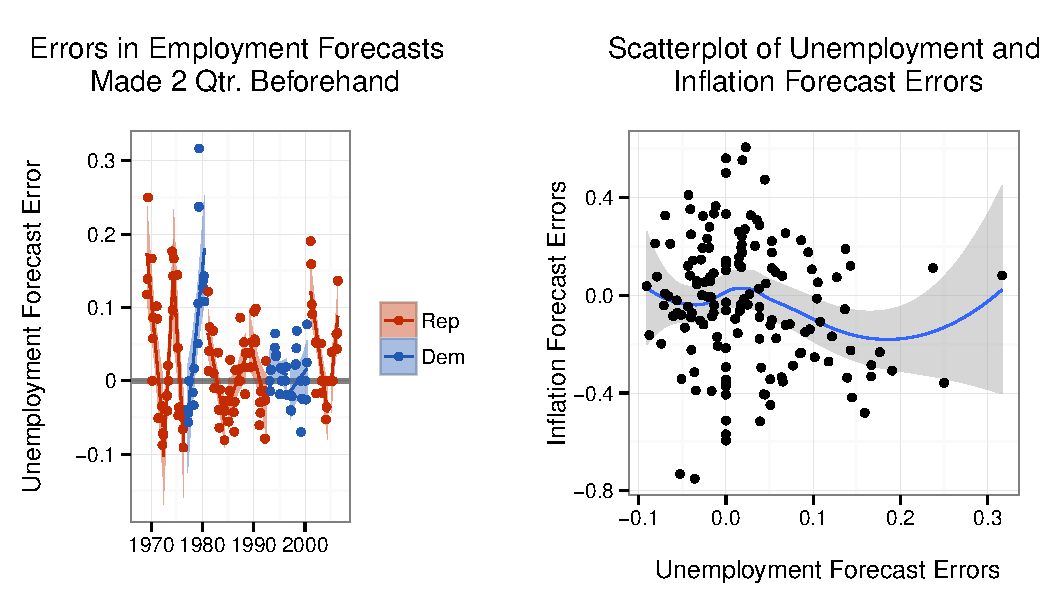
\includegraphics[width=0.95\linewidth]{figure/GraphPartisanErrorUnemploy} 

}



\end{knitrout}


    \end{center}
    \begin{singlespace}
        {\scriptsize{Note: Errors of 0 indicates that inflation/the unemployment rate was perfectly predicted.}}
    \end{singlespace}
\end{figure}

\subsection*{Matching to examine model dependence}

To further examine if our results depend on model specification, rather than an underlying causal effect, we follow recommendations from \cite{Ho2007} to pre-process the data using matching. This data is then used in our parametric regression models to estimate the relationships between our potential causal variables and Fed Staff inflation forecast errors. Doing this allows us to more robustly determine the causal effects of the two `treatments' Fed Staffers are exposed to that we are interested in: a partisan treatment and an electoral treatment.

Pre-analysis matching allows us to mimic the conditions of a randomized experiment. Imagine an ideal world where we could create a controlled experiment to examine the causal relationship between, for example, presidential partisan ID and inflation forecast errors. Following the Neyman-Rubin causal model \citep{Sekhon2008}, estimating causal effects is a comparison between potential outcomes for a hypothetical unit \citep{Stuart2010}. In our study the `unit' is a quarter being forecasted for. The casual effect of presidential party ID on inflation errors is a comparison of the inflation error for the particular quarter when the president is a Democrat and a Republican. We could approach this comparison in an experiment by randomly assigning presidents to quarters. In the language of experimental design the `treatment' could be a Democratic president and the `control' a Republican president. This allows us to have groups of quarters that are as similar as possible except for the president's party ID. Note: in our analysis the determinations of `treatment' and `control' groups is arbitrary.

This is clearly impossible for us. Given that we are working with observational data, other variables that have an impact on forecast errors may have {\emph{different distributions}} across the treatment and control groups \citep{Cochran1973, Diamond2012}. It can be difficult to identify the relationships between presidential party ID, elections, and errors from all of the confounding background variables.

Thus far we have attempted to address this issue statistically with models that allow us to estimate the effect of presidential party ID and elections on forecast errors `controlling for' a wide variety of other factors. However, it may be the case that our results are dependent on the model specifications \citep{Ho2007}. To examine this possibility we aimed to further recreate randomized experimental conditions with pre-analysis matching. We use the {\tt{R}} package {\tt{MatchIt}} \citep{matchit2011} to create two matched data sets where the non-treatment covariates in the control groups closely match those in the treatment groups.

Formally, each quarter $q$ in the data set is `assigned' to either the treatment group ($t_{q} = 1$) or the control group ($t_{q} = 0$). $y_{q}(1)$ is the potential outcome--in our case the inflation forecast error--for quarter $q$ of being in the treatment group, regardless of whether or not it was observed to be in this group. $y_{q}(0)$ is the potential outcome if $q$ was not in the treatment group, regardless of its observed assignment. It is impossible to observe both $y_{q}(1)$ and $y_{q}(0)$ at the same time. Instead we observe one version of $y_{q}=t_{q}y_{q}(1)-(1-t_{q})y_q(0)$. For each $q$ there is a fixed vector of exogenous confounders $X_{q}$. Ideally $t_{q}$ and $X_{q}$ are independent. However, this is not necessarily the case. The point of matching is to reduce or eliminate the relationship between $t_{q}$  and $X_{q}$ by selecting, dropping, and/or duplicating data. Ideally this process matches one treated quarter with one controlled quarter that has the same values of $X_{q}$, i.e. the distribution of covariates is the same in the treated and control groups \citep{matchit2011}. This is known as ``covariate balance" \cite[1]{Diamond2012}. Using matching to balance a data set ``break[s] the link between the treatment variables and the pre-treatment controls'', effectively replicating the conditions of a randomized experiment with observational data \cite[][2--3]{matchit2011}.

Balance is usually achieved in matching with propensity scores: the probabilities that units were assigned the treatment given their covariates. The propensity score model is generally unknown \citep{Drake1993}. To find the propensity score model we use Diamond and Sekhon's \citeyearpar{Diamond2012} genetic matching method (GenMatch).\footnote{The method is implemented with {\tt{MatchIt}}. The original source code for our exact matching models can be found at {\url{http://bit.ly/1gWPhw9}}.} GenMatch is a multivariate method that uses an evolutionary search algorithm to automate the search for the propensity score model that creates maximum balance. This minimizes the difficulty of ``manually and iteratively checking the propensity score" to determine covariate balance \citep[][2]{Diamond2012}.

Once we created the matched data sets we then used them in parametric models similar to those above. See results in tables \ref{OutputEL}, \ref{OutputPL}, and \ref{OutputPB}.

Before discussing the results, let's examine diagnostic tests we ran on the matching models. We primarily diagnosed the matching models with propensity score distribution plots--the probability of a quarter being in the `treated' group given its covariates--as well as quantile-quantile plots to diagnose whether or not each covariate in the matched data sets is balanced \citep{Ho2007}. Please see figures \ref{ElectPropensityScores} and \ref{PresPropensityScores} for the propensity score distributions in our matched data sets. The quantile-quantile plots are not shown, but can easily be created by running the original matching models in our main analysis source code file. The file is available at: \url{http://bit.ly/1gWPhw9}. We are unable to achieve covariate balance for the Congressional interaction terms\footnote{The presidential party ID and election period interaction does balance.} and the Federal Reserve Chair variable. Chairs in our data set in the pre-Volcker/Greenspan era as well as current Chair Ben Bernanke were in office for very few observed quarters, making it difficult to match them. As such, we were not able to test the robustness of our findings for these variables with matched data.

Overall the results are similar when we use matched and non-matched data. The main difference is that the standard errors are larger in models using matched data than unmatched data. See Figure \ref{CoefComparePlots2} for the implications of the larger standard errors. Larger variance is likely because the matched data sample sizes are smaller.

Nonetheless both the point estimates and the uncertainty surrounding our key presidential partisan ID variable are very similar using both matched and non-matched data. We also did not find evidence that inflation forecast errors were associated with elections either independent of presidential party ID or in interaction with it in the matched models, including when we matched based on election period. This provides more evidence that our results are robustly estimating an actual causal effect and are not model dependent.

%%%%%%% Table of  matched data with Normal Linear parametric model %%%%%%%%

\begin{table}[ht]
    \caption{Normal Linear Regression Estimation of Covariate Effects on 2 Qtr. Inflation Forecast Error (Matched by Election Period Variable)}
    \label{OutputEL}
    \vspace{0.25cm}
    \begin{center}
    {\tiny
 
\begin{tabular}{ l D{.}{.}{1}D{.}{.}{1}D{.}{.}{1}D{.}{.}{1}D{.}{.}{1}D{.}{.}{1}D{.}{.}{1}D{.}{.}{1}D{.}{.}{1}D{.}{.}{1}D{.}{.}{1}D{.}{.}{1}D{.}{.}{1} } 
\hline 
  & \multicolumn{ 1 }{ c }{ B1 } & \multicolumn{ 1 }{ c }{ B2 } & \multicolumn{ 1 }{ c }{ B3 } & \multicolumn{ 1 }{ c }{ B4 } & \multicolumn{ 1 }{ c }{ B5 } & \multicolumn{ 1 }{ c }{ B6 } & \multicolumn{ 1 }{ c }{ B7 } & \multicolumn{ 1 }{ c }{ B8 } & \multicolumn{ 1 }{ c }{ B9 } & \multicolumn{ 1 }{ c }{ B10 } & \multicolumn{ 1 }{ c }{ B11 } & \multicolumn{ 1 }{ c }{ B12 } & \multicolumn{ 1 }{ c }{ B13 } \\ \hline
 %                    & B1              & B2              & B3              & B4              & B5              & B6              & B7              & B8              & B9              & B10             & B11             & B12             & B13            \\ 
Intercept            & -0.8            & -0.7            & -0.8            & 5.8 ^\dagger   & 9.1 ^*          & 3.3             & -2.1            & -2.1            & -4.7            & 0.2             & -0.9            & -0.4            & -2.4 ^{***}    \\ 
                     & (4.0)           & (4.0)           & (4.0)           & (3.3)           & (4.0)           & (3.7)           & (4.1)           & (4.1)           & (4.7)           & (3.6)           & (3.7)           & (3.4)           & (0.7)          \\ 
Expenditure/GDP      & 0.2 ^{***}      & 0.2 ^{***}      & 0.2 ^{***}      & 0.2 ^{***}      &                 & 0.2 ^{***}      & 0.2 ^{***}      & 0.2 ^{***}      & 0.2 ^{***}      & 0.2 ^{***}      & 0.2 ^{***}      & 0.1 ^{***}      &                \\ 
                     & (0.0)           & (0.0)           & (0.0)           & (0.0)           &                 & (0.0)           & (0.0)           & (0.0)           & (0.0)           & (0.0)           & (0.0)           & (0.0)           &                \\ 
Output Gap           & -0.0            & -0.0            & -0.0            & -0.1 ^{**}      & -0.1 ^*         & -0.1 ^\dagger  & -0.0            & -0.0            & 0.0             & -0.0            & -0.0            & -0.1            &                \\ 
                     & (0.0)           & (0.0)           & (0.0)           & (0.0)           & (0.0)           & (0.0)           & (0.0)           & (0.0)           & (0.1)           & (0.0)           & (0.0)           & (0.0)           &                \\ 
Discount Rate Change & -0.0            & 0.0             & -0.0            & -0.1            & -0.5 ^*         & -0.1            & -0.2            & -0.2            & -0.3            & 0.1             & 0.1             & 0.3             &                \\ 
                     & (0.2)           & (0.3)           & (0.3)           & (0.2)           & (0.2)           & (0.2)           & (0.2)           & (0.2)           & (0.2)           & (0.2)           & (0.2)           & (0.2)           &                \\ 
Unemployment Rate    & -0.1            & -0.0            & -0.1            & 0.1             & 0.1             & 0.0             & -0.1            & -0.1            & -0.2 ^\dagger  & -0.1            & -0.1            & 0.0             &                \\ 
                     & (0.1)           & (0.1)           & (0.1)           & (0.1)           & (0.1)           & (0.1)           & (0.1)           & (0.1)           & (0.1)           & (0.1)           & (0.1)           & (0.1)           &                \\ 
Qtr. to Election     &                 & 0.0             &                 &                 &                 & 0.0             & 0.0             & 0.0             & -0.0            & 0.0             & 0.0             & 0.0 ^{**}       &                \\ 
                     &                 & (0.0)           &                 &                 &                 & (0.0)           & (0.0)           & (0.0)           & (0.0)           & (0.0)           & (0.0)           & (0.0)           &                \\ 
Qrt. to Election2    &                 & -0.0            &                 &                 &                 &                 &                 &                 & 0.0             &                 &                 &                 &                \\ 
                     &                 & (0.0)           &                 &                 &                 &                 &                 &                 & (0.0)           &                 &                 &                 &                \\ 
Election Period      &                 &                 & -0.0            &                 &                 &                 &                 &                 &                 &                 &                 &                 &                \\ 
                     &                 &                 & (0.1)           &                 &                 &                 &                 &                 &                 &                 &                 &                 &                \\ 
Pres. Party ID       &                 &                 &                 & 0.4 ^{***}      & 0.5 ^{***}      & 0.4 ^{***}      & 0.3 ^{***}      & 0.3 ^{***}      & 0.2             & 1.1 ^{***}      & 1.3 ^{***}      & 11.4 ^{***}     & 6.4 ^*         \\ 
                     &                 &                 &                 & (0.1)           & (0.1)           & (0.1)           & (0.1)           & (0.1)           & (0.1)           & (0.2)           & (0.3)           & (2.7)           & (2.8)          \\ 
Deficit/GDP          &                 &                 &                 &                 & -0.1 ^*         &                 &                 &                 &                 &                 &                 &                 &                \\ 
                     &                 &                 &                 &                 & (0.0)           &                 &                 &                 &                 &                 &                 &                 &                \\ 
FRB/GlobalModel      &                 &                 &                 &                 &                 & 0.1             &                 &                 & 0.0             &                 &                 &                 &                \\ 
                     &                 &                 &                 &                 &                 & (0.1)           &                 &                 & (0.2)           &                 &                 &                 &                \\ 
Senate Dem/Rep       &                 &                 &                 &                 &                 &                 & -0.5 ^*         & -0.5 ^*         & -0.6 ^*         & -0.3            & -0.2            & 1.4 ^\dagger   & 1.1 ^\dagger  \\ 
                     &                 &                 &                 &                 &                 &                 & (0.2)           & (0.2)           & (0.2)           & (0.2)           & (0.2)           & (0.8)           & (0.7)          \\ 
House Dem/Rep        &                 &                 &                 &                 &                 &                 & 0.7 ^{**}       & 0.7 ^{**}       & 0.7 ^*          & 0.7 ^{**}       & 0.6 ^{**}       & 1.6 ^{***}      & 2.1 ^{***}     \\ 
                     &                 &                 &                 &                 &                 &                 & (0.2)           & (0.2)           & (0.3)           & (0.2)           & (0.2)           & (0.4)           & (0.4)          \\ 
Pres*Qrt. Election   &                 &                 &                 &                 &                 &                 &                 &                 & 0.1             &                 &                 &                 &                \\ 
                     &                 &                 &                 &                 &                 &                 &                 &                 & (0.1)           &                 &                 &                 &                \\ 
Pres*Qrt. Election2  &                 &                 &                 &                 &                 &                 &                 &                 & -0.0            &                 &                 &                 &                \\ 
                     &                 &                 &                 &                 &                 &                 &                 &                 & (0.0)           &                 &                 &                 &                \\ 
Pres*House           &                 &                 &                 &                 &                 &                 &                 &                 &                 & -0.6 ^{***}     &                 & -11.6 ^{***}    & -8.1 ^*        \\ 
                     &                 &                 &                 &                 &                 &                 &                 &                 &                 & (0.1)           &                 & (2.7)           & (3.0)          \\ 
Pres*Senate          &                 &                 &                 &                 &                 &                 &                 &                 &                 &                 & -0.8 ^{***}     & -7.0 ^{**}      & -2.0           \\ 
                     &                 &                 &                 &                 &                 &                 &                 &                 &                 &                 & (0.2)           & (2.2)           & (2.1)          \\ 
House*Senate         &                 &                 &                 &                 &                 &                 &                 &                 &                 &                 &                 & -0.9 ^*         & -1.1 ^{**}     \\ 
                     &                 &                 &                 &                 &                 &                 &                 &                 &                 &                 &                 & (0.4)           & (0.4)          \\ 
Pres*House*Senate    &                 &                 &                 &                 &                 &                 &                 &                 &                 &                 &                 & 7.6 ^{***}      & 4.3 ^*         \\ 
                     &                 &                 &                 &                 &                 &                 &                 &                 &                 &                 &                 & (1.9)           & (2.1)           \\
 $N$                  & 61              & 61              & 61              & 61              & 61              & 61              & 61              & 61              & 61              & 61              & 61              & 61              & 61             \\ 
AIC                  & 17.7            & 21.5            & 19.5            & -10.1           & 12.2            & -8.5            & -14.2           & -14.2           & -9.3            & -30.4           & -27.2           & -44.0           & -20.4          \\ 
BIC                  & 59.9            & 80.6            & 70.2            & 40.6            & 62.9            & 59.1            & 61.7            & 61.7            & 100.5           & 54.0            & 57.2            & 65.7            & 47.1           \\ 
$\log L$            & 11.1            & 17.2            & 14.2            & 29.0            & 17.9            & 36.2            & 43.1            & 43.1            & 56.6            & 55.2            & 53.6            & 74.0            & 42.2            \\ \hline
 \multicolumn{14}{l}{\footnotesize{Standard errors in parentheses}}\\
\multicolumn{14}{l}{\footnotesize{$^\dagger$ significant at $p<.10$; $^* p<.05$; $^{**} p<.01$; $^{***} p<.001$}}\\
\multicolumn{14}{l}{\footnotesize{The recession variable is omitted because there was almost no variation in the matched data set.}}\\
\multicolumn{14}{l}{\footnotesize{The reason that there was no variation is because there were only two quarters with both a recession}}\\
\multicolumn{14}{l}{\footnotesize{and an election period in our data set.}} 
\end{tabular} 


    }
    \end{center}
\end{table}

%%%%%%% Table of pres_party matched data with Normal Linear Regression parametric model %%%%%%%%

\begin{table}[ht]
    \caption{Normal Linear Regression Estimation of Covariate Effects on 2 Qtr. Inflation Forecast Error (Matched by President's Party ID variable)}
    \label{OutputPL}
    \vspace{0.25cm}
    \begin{center}
    {\tiny
 
\begin{tabular}{ l D{.}{.}{1}D{.}{.}{1}D{.}{.}{1}D{.}{.}{1}D{.}{.}{1}D{.}{.}{1}D{.}{.}{1}D{.}{.}{1}D{.}{.}{1}D{.}{.}{1}D{.}{.}{1}D{.}{.}{1}D{.}{.}{1} } 
\hline 
  & \multicolumn{ 1 }{ c }{ C1 } & \multicolumn{ 1 }{ c }{ C2 } & \multicolumn{ 1 }{ c }{ C3 } & \multicolumn{ 1 }{ c }{ C4 } & \multicolumn{ 1 }{ c }{ C5 } & \multicolumn{ 1 }{ c }{ C6 } & \multicolumn{ 1 }{ c }{ C7 } & \multicolumn{ 1 }{ c }{ C8 } & \multicolumn{ 1 }{ c }{ C9 } & \multicolumn{ 1 }{ c }{ C10 } & \multicolumn{ 1 }{ c }{ C11 } & \multicolumn{ 1 }{ c }{ C12 } & \multicolumn{ 1 }{ c }{ C13 } \\ \hline
 %                    & C1              & C2              & C3              & C4              & C5              & C6              & C7              & C8              & C9              & C10             & C11             & C12             & C13            \\ 
Intercept            & 2.2             & 1.7             & 2.1             & 2.6             & -2.5            & 2.2             & -5.2            & -5.2            & -6.4            & -4.2            & -5.2            & -2.0            & 1.9            \\ 
                     & (4.2)           & (4.3)           & (4.2)           & (3.5)           & (3.5)           & (3.6)           & (4.3)           & (4.3)           & (4.9)           & (4.0)           & (4.1)           & (4.3)           & (1.8)          \\ 
Recession            & 0.2             & 0.2             & 0.2             & 0.1             & 0.0             & 0.2             & 0.1             & 0.1             & 0.1             & 0.2             & 0.1             & 0.2             &                \\ 
                     & (0.2)           & (0.2)           & (0.2)           & (0.2)           & (0.2)           & (0.2)           & (0.2)           & (0.2)           & (0.2)           & (0.1)           & (0.1)           & (0.2)           &                \\ 
Expenditure/GDP      & 0.1 ^*          & 0.1 ^*          & 0.1 ^*          & 0.2 ^{**}       &                 & 0.2 ^{**}       & 0.2 ^{***}      & 0.2 ^{***}      & 0.2 ^{***}      & 0.1 ^*          & 0.2 ^{**}       & 0.1             &                \\ 
                     & (0.1)           & (0.1)           & (0.1)           & (0.0)           &                 & (0.0)           & (0.1)           & (0.1)           & (0.1)           & (0.1)           & (0.0)           & (0.1)           &                \\ 
Output Gap           & -0.0            & -0.0            & -0.0            & -0.1            & 0.0             & -0.1            & 0.0             & 0.0             & 0.0             & 0.0             & 0.0             & 0.0             &                \\ 
                     & (0.1)           & (0.1)           & (0.1)           & (0.0)           & (0.0)           & (0.0)           & (0.0)           & (0.0)           & (0.1)           & (0.0)           & (0.0)           & (0.0)           &                \\ 
Discount Rate Change & -0.5            & -0.6 ^\dagger  & -0.6 ^\dagger  & -0.6 ^*         & -0.7 ^*         & -0.5 ^\dagger  & -0.5 ^\dagger  & -0.5 ^\dagger  & -0.5 ^\dagger  & -0.2            & -0.2            & -0.4            &                \\ 
                     & (0.3)           & (0.3)           & (0.3)           & (0.3)           & (0.3)           & (0.3)           & (0.2)           & (0.2)           & (0.3)           & (0.2)           & (0.3)           & (0.3)           &                \\ 
Unemployment Rate    & -0.0            & -0.0            & -0.0            & -0.0            & -0.1            & -0.0            & -0.2 ^*         & -0.2 ^*         & -0.2            & -0.1            & -0.1            & -0.2            &                \\ 
                     & (0.1)           & (0.1)           & (0.1)           & (0.0)           & (0.1)           & (0.1)           & (0.1)           & (0.1)           & (0.1)           & (0.1)           & (0.1)           & (0.1)           &                \\ 
Qtr. to Election     &                 & 0.0             &                 &                 &                 & 0.0             & 0.0             & 0.0             & 0.0             & 0.0             & 0.0             & 0.0             &                \\ 
                     &                 & (0.0)           &                 &                 &                 & (0.0)           & (0.0)           & (0.0)           & (0.1)           & (0.0)           & (0.0)           & (0.0)           &                \\ 
Qrt. to Election2    &                 & -0.0            &                 &                 &                 &                 &                 &                 & -0.0            &                 &                 &                 &                \\ 
                     &                 & (0.0)           &                 &                 &                 &                 &                 &                 & (0.0)           &                 &                 &                 &                \\ 
Election Period      &                 &                 & -0.1            &                 &                 &                 &                 &                 &                 &                 &                 &                 &                \\ 
                     &                 &                 & (0.1)           &                 &                 &                 &                 &                 &                 &                 &                 &                 &                \\ 
Pres. Party ID       &                 &                 &                 & 0.3 ^{***}      & 0.4 ^{***}      & 0.3 ^{***}      & 0.4 ^{***}      & 0.4 ^{***}      & 0.3             & 1.2 ^{***}      & 1.2 ^{**}       & -1.3            & -1.6           \\ 
                     &                 &                 &                 & (0.1)           & (0.1)           & (0.1)           & (0.1)           & (0.1)           & (0.3)           & (0.3)           & (0.4)           & (2.2)           & (1.9)          \\ 
Deficit/GDP          &                 &                 &                 &                 & -0.1            &                 &                 &                 &                 &                 &                 &                 &                \\ 
                     &                 &                 &                 &                 & (0.0)           &                 &                 &                 &                 &                 &                 &                 &                \\ 
FRB/GlobalModel      &                 &                 &                 &                 &                 & -0.1            &                 &                 & -0.1            &                 &                 &                 &                \\ 
                     &                 &                 &                 &                 &                 & (0.1)           &                 &                 & (0.1)           &                 &                 &                 &                \\ 
Senate Dem/Rep       &                 &                 &                 &                 &                 &                 & -1.3 ^{**}      & -1.3 ^{**}      & -1.1 ^*         & -0.8 ^*         & -0.7 ^\dagger  & -3.7            & -3.8 ^\dagger \\ 
                     &                 &                 &                 &                 &                 &                 & (0.4)           & (0.4)           & (0.4)           & (0.4)           & (0.4)           & (2.4)           & (2.0)          \\ 
House Dem/Rep        &                 &                 &                 &                 &                 &                 & 1.1 ^{**}       & 1.1 ^{**}       & 1.0 ^*          & 1.2 ^{***}      & 1.0 ^{**}       & -0.1            & -0.9           \\ 
                     &                 &                 &                 &                 &                 &                 & (0.3)           & (0.3)           & (0.4)           & (0.3)           & (0.3)           & (1.5)           & (1.4)          \\ 
Pres*Qrt. Election   &                 &                 &                 &                 &                 &                 &                 &                 & 0.0             &                 &                 &                 &                \\ 
                     &                 &                 &                 &                 &                 &                 &                 &                 & (0.1)           &                 &                 &                 &                \\ 
Pres*Qrt. Election2  &                 &                 &                 &                 &                 &                 &                 &                 & -0.0            &                 &                 &                 &                \\ 
                     &                 &                 &                 &                 &                 &                 &                 &                 & (0.0)           &                 &                 &                 &                \\ 
Pres*House           &                 &                 &                 &                 &                 &                 &                 &                 &                 & -0.7 ^*         &                 & -0.3            & 0.1            \\ 
                     &                 &                 &                 &                 &                 &                 &                 &                 &                 & (0.2)           &                 & (1.7)           & (1.6)          \\ 
Pres*Senate          &                 &                 &                 &                 &                 &                 &                 &                 &                 &                 & -0.8 ^*         & 4.1             & 4.5 ^*         \\ 
                     &                 &                 &                 &                 &                 &                 &                 &                 &                 &                 & (0.4)           & (2.9)           & (2.1)          \\ 
House*Senate         &                 &                 &                 &                 &                 &                 &                 &                 &                 &                 &                 & 1.8             & 2.3            \\ 
                     &                 &                 &                 &                 &                 &                 &                 &                 &                 &                 &                 & (1.7)           & (1.5)          \\ 
Pres*House*Senate    &                 &                 &                 &                 &                 &                 &                 &                 &                 &                 &                 & -1.7            & -2.2           \\ 
                     &                 &                 &                 &                 &                 &                 &                 &                 &                 &                 &                 & (1.8)           & (1.5)           \\
 $N$                  & 54              & 54              & 54              & 54              & 54              & 54              & 54              & 54              & 54              & 54              & 54              & 54              & 54             \\ 
AIC                  & 11.5            & 14.0            & 12.4            & -7.2            & 3.6             & -4.1            & -14.4           & -14.4           & -10.0           & -20.8           & -18.2           & -18.1           & -18.4          \\ 
BIC                  & 59.2            & 77.7            & 68.1            & 48.5            & 59.3            & 67.5            & 65.1            & 65.1            & 101.4           & 66.7            & 69.3            & 93.3            & 45.3           \\ 
$\log L$            & 18.3            & 25.0            & 21.8            & 31.6            & 26.2            & 38.1            & 47.2            & 47.2            & 61.0            & 54.4            & 53.1            & 65.0            & 41.2            \\ \hline
 \multicolumn{14}{l}{\footnotesize{Standard errors in parentheses}}\\
\multicolumn{14}{l}{\footnotesize{$^\dagger$ significant at $p<.10$; $^* p<.05$; $^{**} p<.01$; $^{***} p<.001$}} 
\end{tabular} 


    }
    \end{center}
\end{table}

%%%%%%% Table of pres_party matched data with Normal Bayesian linear parametric model %%%%%%%%

% latex table generated in R 3.1.0 by xtable 1.7-3 package
% Fri May  9 09:40:54 2014
\begin{table}[ht]
\centering
\caption{Bayesian Normal Linear Regression Estimation of Covariate Effects on 2 Qtr. Inflation Forecast Error (Matched by President's Party ID variable)} 
\label{OutputPB}
{\small
\begin{tabular}{lccccc}
  \hline
Variables & Mean & SD & 2.5\% & 50\% & 97.5\% \\ 
  \hline
Intercept & 2.17 & 3.64 & -4.84 & 2.15 & 9.57 \\ 
  Pres. Party ID & 0.33 & 0.07 & 0.19 & 0.33 & 0.48 \\ 
  Recession & 0.16 & 0.17 & -0.17 & 0.16 & 0.49 \\ 
  Qtr. to Election & 0.00 & 0.01 & -0.01 & 0.00 & 0.02 \\ 
  Expenditure/GDP & 0.16 & 0.05 & 0.06 & 0.16 & 0.25 \\ 
  Output Gap & -0.06 & 0.04 & -0.14 & -0.05 & 0.03 \\ 
  Discount Rate Change & -0.54 & 0.29 & -1.11 & -0.54 & 0.02 \\ 
  Unemployment Rate & -0.00 & 0.06 & -0.12 & -0.00 & 0.11 \\ 
  Global Model & -0.07 & 0.10 & -0.26 & -0.07 & 0.11 \\ 
  sigma2 & 0.05 & 0.01 & 0.03 & 0.05 & 0.07 \\ 
   \hline
\end{tabular}
}
\end{table}



%%%%%%% Matching Diagnostic Plots %%%%%%
%%%%% Elections %%%%%%%
\begin{figure}[h]
  \caption{Matched on Election Period}
  \label{ElectPropensityScores}
\begin{knitrout}
\definecolor{shadecolor}{rgb}{0.969, 0.969, 0.969}\color{fgcolor}

{\centering 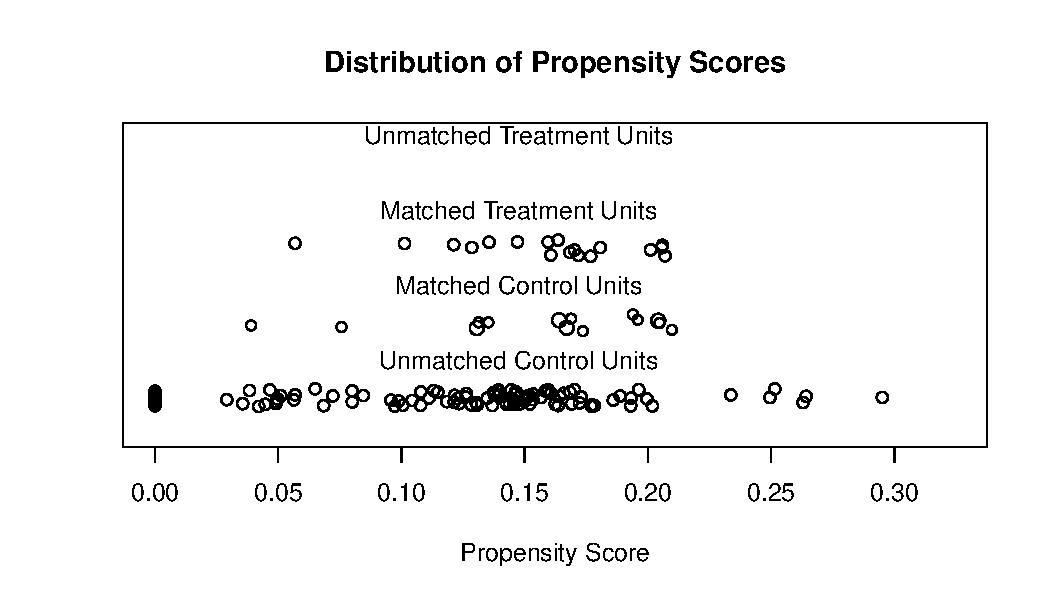
\includegraphics[width=\maxwidth]{figure/ElectPropensity} 

}



\end{knitrout}

    \begin{singlespace}
        {\scriptsize{Pre- and Post-matching propensity scores, where the ``Treated Units" are election quarters or the quarter before. ``Control Units" are from all other quarters. The more similar the distribution of matched treated and control unit propensity scores, the more successful the matching model was \cite[17]{Hollyer2012}.}}
    \end{singlespace}
\end{figure}

%%%%% Presidential Party ID %%%%%%
\begin{figure}[h]
  \caption{Matched on Presidential Party Identification}
  \label{PresPropensityScores}
\begin{knitrout}
\definecolor{shadecolor}{rgb}{0.969, 0.969, 0.969}\color{fgcolor}

{\centering 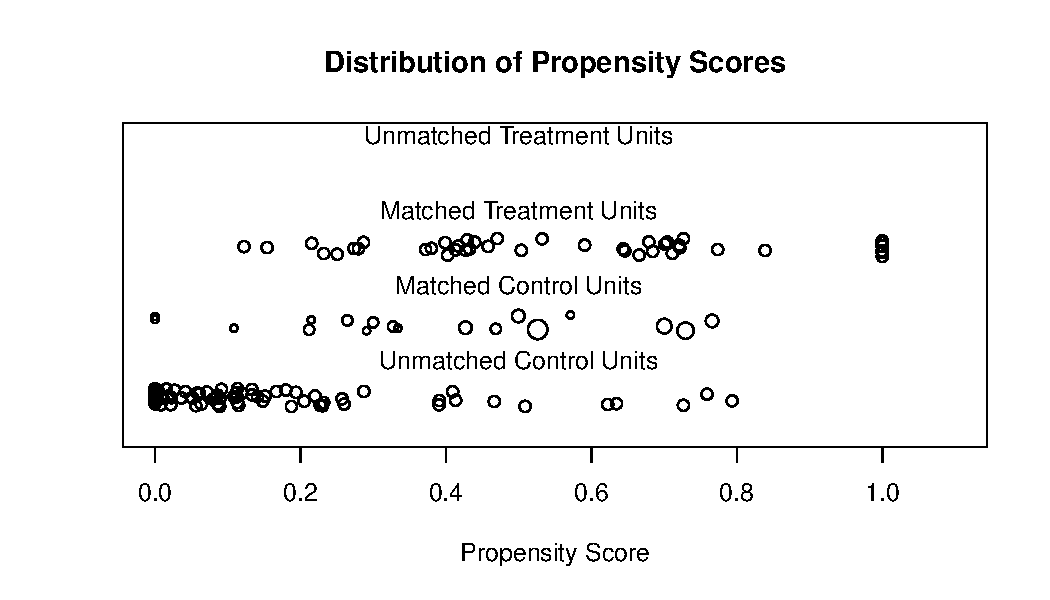
\includegraphics[width=\maxwidth]{figure/PresPropensity} 

}



\end{knitrout}

  \begin{singlespace}
      {\scriptsize{Pre- and Post-matching propensity scores, where the ``Treated Units" are quarters when the president was a Democrat. ``Control Units" are quarters when with a Republican president. The more similar the distributions of matched treated and control unit propensity scores, the more successful the matching model was \cite[17]{Hollyer2012}.}}
  \end{singlespace}
\end{figure}

\begin{figure}[t]
    \caption{95\% Confidence Bands for Coefficients from a Variety of Matching and Parametric Model Specifications}
    \label{CoefComparePlots2}
    \begin{center}

\begin{knitrout}
\definecolor{shadecolor}{rgb}{0.969, 0.969, 0.969}\color{fgcolor}

{\centering \includegraphics[width=0.95\linewidth]{figure/CoefComparePlotsMatched} 

}



\end{knitrout}

    \end{center}
    \begin{singlespace}
        {\scriptsize{Data matched by presidential party identification. Intercept values are not shown to maintain a reasonable scale for comparing covariate estimates.}}
    \end{singlespace}
\end{figure}

\subsection*{A brief history of inflation forecasting models at the US Federal Reserve (1970-2013)}

Beginning in 1970 the Federal Reserve\footnote{As before, this discussion draws heavily on Brayton et al.'s \citeyear{Brayton1997} detailed description of the changes to Federal Reserve forecasting models that took place in 1996.} implemented its first comprehensive statistical forecasting model of US Economy, generally known as the MPS.\footnote{MPS stands for MIT-Penn-SSRC, the economics departments associated with the original contributors to the model used by the Fed.} This model contained 60 behavioral equations solved simultaneously in which short-run dynamics were based on an IS/LM/Phillips Curve paradigm while long-run dynamics were given by the neoclassical growth model of production, factor demands, and consumption. In 1975, the Fed responded to the first oil shock and the dissolution of Bretton Woods by creating the Multi-Country Model (MCM) to estimate economic inter-dependencies between the US and other major economic powers. The MCM contained over 200 behavioral equations and was based on similar assumptions about the relationship between inflation and unemployment, and so on as the MPS model. Expectations in both the MPS and the MCM were modeled as adaptive and often subsumed through independent variable lags. The use of adaptive expectations meant that actors were inherently backward-looking, incorporating old information into future behavior, but failing to account for expected future outcomes in current behavior. Adaptive expectations would be the defining feature of Federal Reserve forecasts through 1995 \citep[45]{Brayton1997}. Equations and variables were changed over the 25 years that the MPS and MCM models were in use to adjust for new macroeconomic knowledge, but these changes did not alter the basic structure of the models. Furthermore, these minor changes were incremental and not documented in a unified framework, at least not in a way that is accessible to researchers. Attempts to account for these minor changes explicitly in our models would be at best atheoretical and at worst impossible.

It wasn't until 1996 that the fundamental assumptions of the model were changed in response to the rise of rational expectations theories in economics. The incorporation of rational expectations into the forecasts required a completely new set of models that are self-referential and internally consistent. That is, predictions made by the model are used as expected outcomes in other equations in an iterative manner until estimates converge. Market actors in these new models (FRB/US and FRB/Global) are forward-looking: making investment, spending, and production decisions based on expectations of future economic outcomes. The adjustments they make to their behavior in response to these expectations then alter likely outcomes, which must then be accounted for in the estimates, and so on. The fundamental difference between the MPS-MCM and FRB/US-FRB/Global frameworks is that while the older forecasting models assumed that market participants would extrapolate recent economic outcomes into the future, the new models assume that actors respond strategically to these extrapolations by altering their behavior which can in turn alter expected outcomes.


%%%%%%% References %%%%%%%%%%%%

\clearpage

\bibliographystyle{apsr}
\bibliography{GreenBook.bib}

\end{document}
